\documentclass[11pt]{article}
\usepackage[utf8]{inputenc}
\usepackage[T1]{fontenc}
\usepackage{tgbonum}
\usepackage[english]{babel}
\usepackage{natbib}
\usepackage{enumerate}
\usepackage[shortlabels]{enumitem}
\usepackage{subcaption}
\usepackage{subfloat}
\usepackage{graphicx}
\usepackage{hyperref}
\usepackage{amsbsy}
\usepackage{gensymb}
\usepackage
[
a4paper,
left=2.5cm,
right=2.5cm,
top=2cm,
bottom=2cm,
]{geometry}
\usepackage{fancyhdr}
\pagestyle{fancy}
\fancyhf{}
\rfoot{\thepage}
\renewcommand{\headrulewidth}{0pt}
\usepackage{charter}
\usepackage{color}
\definecolor{code-pink}{RGB}{199, 37, 78}

\begin{document}

\begin{center}

	\vspace{5ex}
    \fontsize{20}{10}\selectfont {Modal analysis of a dynamical system using Proper Orthogonal Decomposition (POD) and Dynamic Mode Decomposition (DMD)}

\vskip1ex

{\rule{\textwidth}{0.5pt}}

  \end{center}
  
\section*{Project description}

The aim of this project is to apply the POD and the DMD to analyse a dynamical system. POD \cite{Berkooz1993} (also known as PCA or KLT) is a decomposition technique which aims at finding the structure in the dataset associated with the maximum energy. It is often used in the construction of Reduced Order Models (ROMs), because it allows the reduction of the system's dimensionality. \par
The POD is generally performed by applying the singular value decomposition to the dataset:
\begin{equation}
	\mathbf{X} = \mathbf{U} \mathrm{\boldsymbol{\Sigma}} \mathbf{V}^{T}
\end{equation}where $\mathbf{X}$ is the data matrix, $\mathbf{U}$ and $\mathbf{V}$ contain the spatial and temporal modes, and $\mathrm{\boldsymbol{\Sigma}}$ is a diagonal matrix containing the singular values. \par
The goal of DMD \cite{Tu2014} is to find the best linear representation of a dynamical system. This is achieved by computing the linear operator $\mathbf{A}$ such that:
\begin{equation}
\mathbf{x}_{k + 1} = \mathbf{A} \ \mathbf{x}_{k}
\end{equation}where $\mathbf{x}_{k}$ and $\mathbf{x}_{k + 1}$ represent the state of the system at time $k$ and $k+1$. The DMD modes are the eigenvectors of matrix $\mathbf{A}$, while the eigenvalues of $\mathbf{A}$ are linked to the frequency of the DMD modes. \par
The objective of this work is to apply POD and DMD to two different dynamical systems: the first one is a simple damped harmonic oscillator, while the second one is represented by the flow past a cylinder. In both cases, the solution should include a critical assessment of the POD and DMD modes retrieved, highlighting the pros and cons of one approach over the other.

\section*{Tasks}

In this project, you will complete the following tasks:

\begin{enumerate}[start=1,label={\bfseries Task \arabic*:}]
\item The damped harmonic oscillator is a simple dynamical system in which the forces experienced by the mass are the restoring force of the spring and the dampening force of friction:
\begin{equation}
m\frac{d^2s}{dt^2} + c \frac{ds}{dt} + ks = 0
\end{equation}where $m$ is the mass, $c$ is the dampening coefficient, $k$ is the spring constant and $s$ is the axis of movement. The system has an analytic solution:
\begin{equation}
s(t) = A_0e^{-c/2m \ t}\cos(\omega t + \phi) 
\end{equation}where $A_0$ and $\phi$ depend on the initial conditions and $\omega = \sqrt{k/m - (c/2m)^2}$. \par
The steps to solve the first exercise are:
\begin{itemize}
\item  Construct an underdamped ($c < \sqrt{4 m k}$) harmonic oscillator with your choice of characteristic frequency and starting conditions.
\item Build a synthetic dataset by pretending that the position of the mass is tracked in time by two sensors in the $x, y$ directions. Each sensor has a 5\% uncertainty (random white noise) and the angle between the $s$ and $x$ axis is equal to $\theta = 35 \degree$, as reported in Fig. \ref{fig_spring_experiment}. Collect the position for $6 \ \tau$ , where $\tau = 2m/c$ is the characteristic time length. 

\begin{figure}[h]
\centering
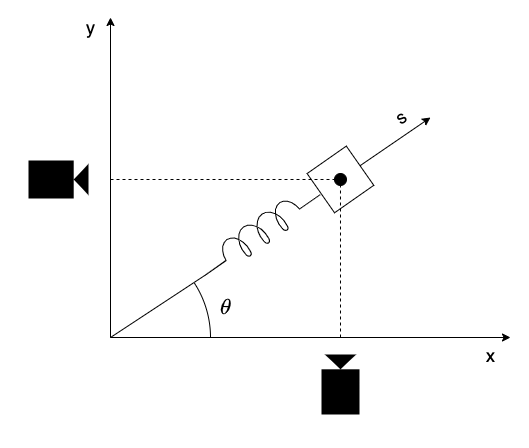
\includegraphics[width=4in]{Images/Spring_experiment.png}
\caption{Sketch of the virtual experiment.}
\label{fig_spring_experiment} 
\end{figure}

\item Apply the POD and DMD algorithms to the data matrix $\mathbf{X}$ containing the $x$ and $y$ positions. To perform the POD and DMD, you can use the python libraries that you can find \href{https://github.com/mendezVKI/MODULO}{here}, along with the instruction for the installation and the documentation.
\item Compare the POD and DMD results. 
\end{itemize}
\item The Reynolds number is an adimensional number which quantifies the tendency of the flow to display a chaotic (turbulent) behaviour:
\begin{equation}
Re = v D/ \nu
\end{equation}
where $v$ is the flow velocity, $D$ is the cylinder diameter and $\nu$ is the kinematic viscosity. After a critical $Re$, the wake of a cylinder immersed in a flow displays the Von Karman instability, which is characterized by an asymmetric vortex shedding with an intrinsic frequency. This frequency depends on the velocity of the flow and on the characteristic length of the cylinder, and it is usually reported as the adimensional Strohual number $St = f_{VK} D/ v$, where $f_{VK}$ is the frequency of the Von Karman instability. The $St$ for the Von Karman instability is around 0.2.\par
The steps to follow to solve the exercise are:
\begin{itemize}
\item Download the data of the numerical simulation of the flow past the cylinder from \href{http://dmdbook.com/}{here}, by clicking on \verb|DATA.zip|. The simulation is performed for 151 timesteps, and the grid has dimensions $449 \times 199 $. The simulation was performed using the IBMP code based on immersed boundary method of Taira and Colonius \cite{Taira2007}.
Inside the folder \verb|DATA|, go to the directory \verb|FLUIDS|. Here, you will find the data in the matlab file \verb|CYLINDER_ALL.mat|, for the axial velocity (UALL), radial velocity (VALL) and vorticity (VORTALL). The matrix of each quantity is organized as a $(449 \cdot 199) \times 151 $ matrix, where each column represents one time step of the simulation. To visualize a single time step, the column has to be reshaped into a $449 \times 199$ matrix. \par 
If you use python, you can export the data in a file \verb|.csv| and import it on your code.  
\item Apply the POD and DMD algorithms to the vorticity dataset as in the previous task.
\item (\textit{Optional}) Apply the POD and DMD algorithms to matrix containing both the axial and radial velocity.
\item Compare the results.

\end{itemize}
\end{enumerate}

\section*{Written report}

Your written report should contain the following:

\begin{enumerate}[start=1,label={\bfseries Section \arabic*:}]
\item A brief introduction of the mathematical formulation of POD and DMD. In particular, highlight the computational advantages and drawbacks of the two techniques.
\item Results corresponding to \textbf{Tasks 1}, compared to the analytical solution.
\item Results corresponding to \textbf{Tasks 2}, including relevant figures and a discussion of the differences between POD and DMD.
\item Final discussion and conclusions, highlighting the role of these decomposition techniques in the study of dynamical systems. Don't forget to cite the relevant literature to strengthen your conclusions. 
\end{enumerate}

\section*{Resources}

You can find a series of introductory videos on modal analysis from Pr. Mendez \href{https://www.youtube.com/channel/UC-RoU7LisZSLy6o-EO4BUDA/playlists}{here}. The papers introducing POD and DMD are cited in the bibliography. If you encounter problems in the download of the data or installation of the libraries you can contact Alberto Procacci on TEAMS or at alberto.procacci@ulb.be.

\bibliographystyle{unsrt}
\bibliography{bib}

\end{document}